\chapter{Objectives Specification and Work Environment}

\section*{Introduction}
This chapter will first define the project's functional and non-functional requirements, then we will discuss the chosen structural deceisions , explaining the reasoning behind their selection. Finally we will specify the hardware and software resources necessary for this project.

\section{Project Specification}
Requirements analysis is a fundamental phase in every project realization process. It is based on the study of the project's features as well as the constraints. In this section, we will cover both the functional and non-functional requirements.

\subsection{Functional Requirements}

The goal of the project is to generate a running CoreMark project on STM32 devices using CMSIS-Toolbox in an automated way. Within this context, this means guaranteeing the following concepts:

%\begin{itemize}
%    \item \textbf{Automation:} Ensuring that the user can generate a ready-to-build project without manually setting up peripheral configurations or memory layouts.
%    \item \textbf{Device Adaptability:} The project template must be dynamic in order to accomodate for the device specific characteristics of STM32 MCUs.
%    \item \textbf{CoreMark Integration:} CoreMark must be pre-configured and integrated within the project so that it can be executed immediately without further setup.
%    \item \textbf{Result Reporting:} The CoreMark results must be ouput in a standardized format, enabling consistent performance comparisons between devices.
%    \item \textbf{Multi-Toolchain Support:} The user should be able to build the project using any of the main embedded systems compilers without any extra configuration steps.
%\end{itemize}
%
%Table \ref{tab:functional_requirements} neatly summarizes the functional requirements for our project.

\begin{table}[htbp]
    \centering
    \caption{Functional Requirements for CMSIS-Toolbox based automated benchmarking}
    \label{tab:functional_requirements}
    \begin{tabularx}{\linewidth}{@{}>{\bfseries}l X X@{}}
        \toprule
        Requirements & Description \\
        \midrule
        Automation & The system must automatically generate a CoreMark benchmarking project for STM32 devices without requiring manual configuration. \\ \midrule
        Device Adaptability & The generated project must adapt to different STM32 families and configurations. \\ \midrule
        CoreMark Integration & The CoreMark benchmark must be integrated and ready to run immediately on the target hardware. \\ \midrule
        Result Reporting & The system must provide a standardized mechanism for reporting benchmark results. \\ \midrule
        Multi-Toolchain Support & The project must support multiple compilers such as GCC, ARM Compiler, and IAR. \\ \bottomrule
    \end{tabularx}
\end{table}
\subsection{Non-Functional Requirements}
Below are the non-functional requirements or the constraints that the functional expectations must abide by:
\begin{itemize}
    \item \textbf{Performance Requirements:}
    \begin{itemize}
        \item \textbf{Low Overhead} The project must not add significant, if any overhead besides the CoreMark runtime, this insures the integrity of the benchmarking results.
        \item \textbf{Compiler Optimizations} The project must provide the most optimal compiler configuration to ensure the maxmium performance results.
    \end{itemize}
   \item \textbf{Reliability Requirements:}
   \begin{itemize}
    \item \textbf{Correctness} The project must be functional and able to run without manual fixes.
    \item \textbf{Consistency} The project must produce consistent results amongst STM32 devices.
    \item \textbf{Error Handling} The project must fail gracefully and generate meaningful error messages.
   \end{itemize}
   \item \textbf{Usability Requirements:}
   \begin{itemize}
    \item \textbf{Ease of use} The generation process must be simple and intuitive, the project structure must be clear and consistent.
    \item \textbf{Standardized Output} The results must be presented in a clear format to facilitate further automation and data collection.
   \end{itemize}
\end{itemize}

\section{Structural Decisions}
Before delving further into the implementation details, it is crucial to understand the rationale behind the structural decisions chosen, for both the generation tool and the CoreMark project. This sections elucidates the reasons behind the choices and their relevence to the project's objectives.
\subsection{CoreMark Project}
The CoreMark project is the end result of the generation tool, it is meant to be runnable out of the box with the 3 main compilers (GCC, ARM, and IAR).

Ensuring the cross-toolchain support is done by providing the necessary compiler specific directives:
\begin{itemize}
	\item \textbf{Linker Scripts}
	Each compiler has their own unique format for linker scripts:
	\begin{itemize}
		\item \textbf{GCC:} GCC uses the .ld file extension and the LDScript syntax for the linking phase, it is structued in a declarative way to generate regions, sections and describe behavior within elements as well as exporting symbols.
		\item \textbf{IAR:} IAR uses the .icf file extension as well as proprietary syntax for the linking phase, it allows the user to simply declare regions and optionally sections and takes care of the rest.
		\item \textbf{ARM:} ARM compiler uses the .sct file extension, you only have to declare memory regions and the rest is handled either in C code or by the compiler directly.
	\end{itemize}
	\item \textbf{Startup Files} The startup file is written in assembly (This approach is changed in HAL2), and although most of the code is common between the 3 compilers, some specific instructions/symbols are different, as well as the libc initialization function is different as each compiler uses a different implementation.
	\item \textbf{Compiler Options} Each compiler has their own set of compiler flags to be used, providing each one with the appropriate configuration is crucial to ensure consistent running.
	\item \textbf{Generic Print Function Implementation} As mentioned prior, each compiler uses a different implementation of libc, meaning that the syscall behind the standard library's printf function are different, providing our own implementation and passing it to CoreMark for result reporting is the most efficient and platform-agnostic solution.
\end{itemize}
The table \ref{tab:cm_prj_struct} provides an overview of the architecture of the CoreMark project.
\begin{table}[H]
	\centering
   	\caption{CoreMark Project Structure}
   	\label{tab:cm_prj_struct}
   	\begin{tabularx}{\linewidth}{@{}>{\bfseries}l X X@{}}
    \toprule
    Element & Description \\
    \midrule
    User Code & This component provides the definition for the user application's entry point as well as the UART peripheral configuration. \\
    \midrule
    Driver & This component includes the necessary HAL drivers to enable the UART peripheral. \\
    \midrule
    Toolchain\_Specific & This component contains the toolchain specific source and header files to modify if the user wants to modify system configurations such as linker scripts and startup files. \\
    \midrule
    CoreMark & This component contains the source code of the CoreMark benchmark to be invoked within the usercode's entry point. \\
    \midrule
    coremark.csolution.yml & This is the workspace file for CMSIS-Toolbox to have knowledge of the project, it defines the DFP, ARM's CORE component, alongside the target device, build types and compiler selection. \\
    \midrule
    coremark.cproject.yml & This is the project description file, it contains the source files to be compiled, user defines for UART functionality and the include paths. \\
    \midrule
    cdefault.yml & This is the file that contains all the compiler options, in our context, the configuration is meant to provide the most performance-oriented setup. \\
    \bottomrule
   \end{tabularx}
\end{table}


\subsection{Project Generation Tool}
The architecture of the CoreMark project is quite complex and contains multiple pieces that must be either generated dynamically or fetched from different resources.
\begin{figure}[H]
    \centering
    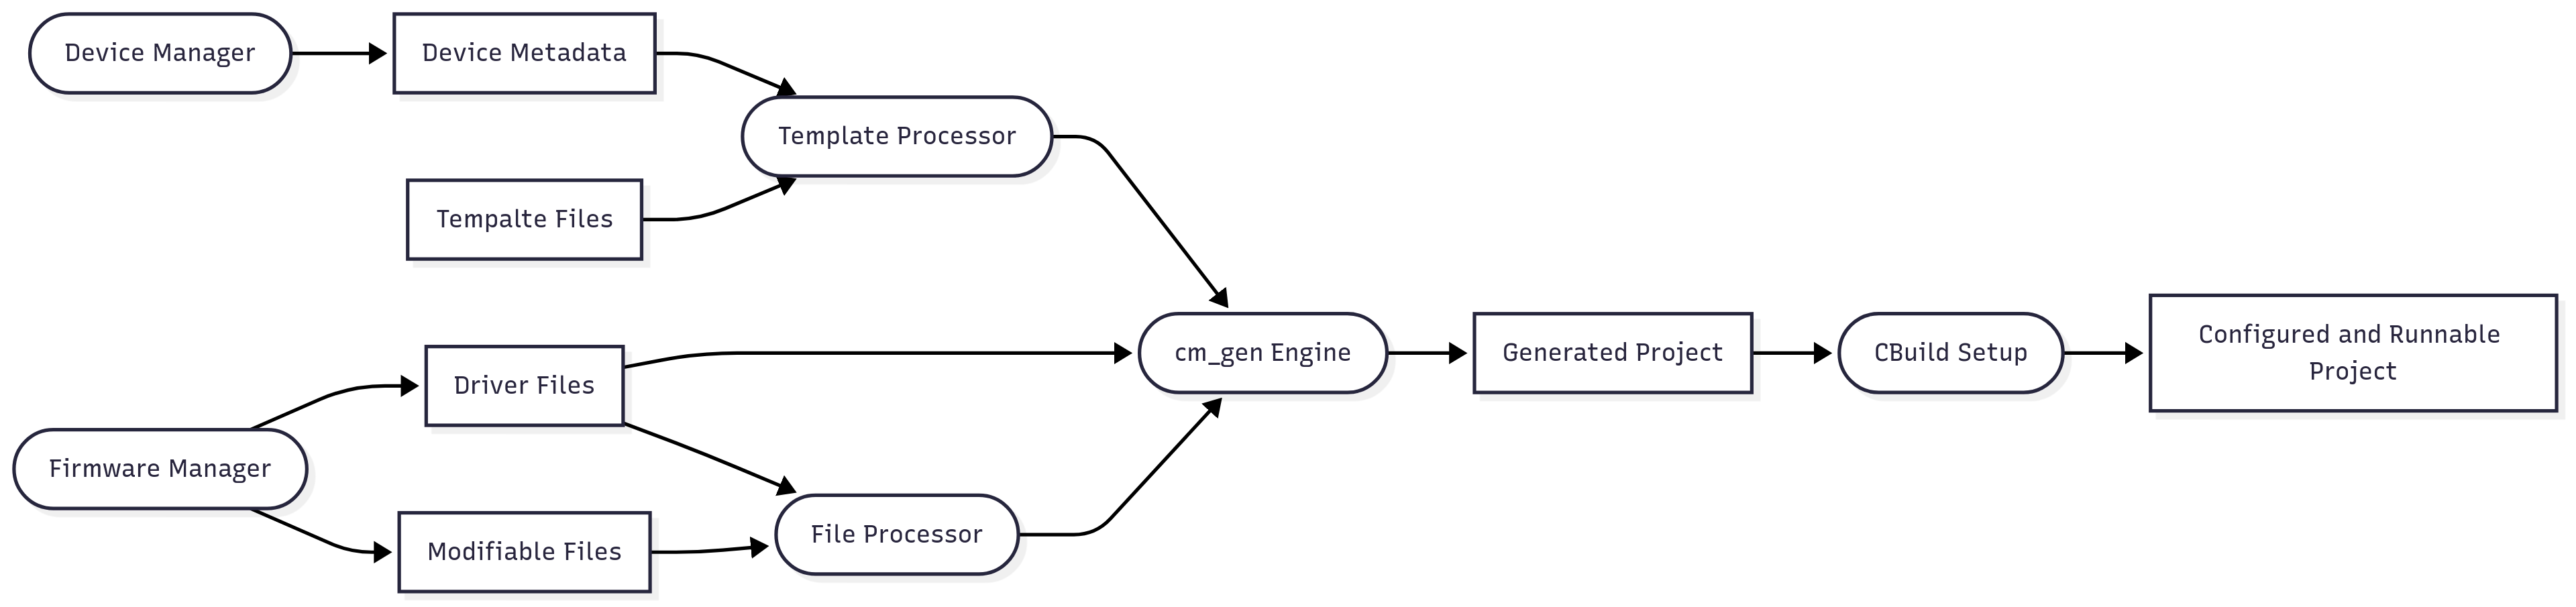
\includegraphics[width=15cm]{ST_Summer_Internship/GenerationToolComponents.png}
    \caption{Project Generation Tool Architecture}
    \label{fig:gen_tool_arch}
\end{figure}
The figure \ref{fig:gen_tool_arch} shows the multiple modules within the project generation tool.
\begin{table}[htbp]
   \centering
   \caption{Project Generation Tool Structure}
   \begin{tabularx}{\linewidth}{@{}>{\bfseries}l X X@{}}
    \toprule
    Module & Description \\
    \midrule
       Device Manager & Extracts the device metadata \\
    \midrule
       Firmware Manager & Manages the device's firmware pack and extracting the necessary files \\
    \midrule
       Template Processor & Generates files from the template files and the gathered data \\
    \midrule
       File Processor & Modifies firmware files that cannot be templated to accomodate for our project's context \\
    \midrule
       cm\_gen Engine & Orchestrates and runs the different modules \\
    \bottomrule
   \end{tabularx}
\end{table}

\section{Use-Case Diagram}

\begin{figure}[H]
	\centering
	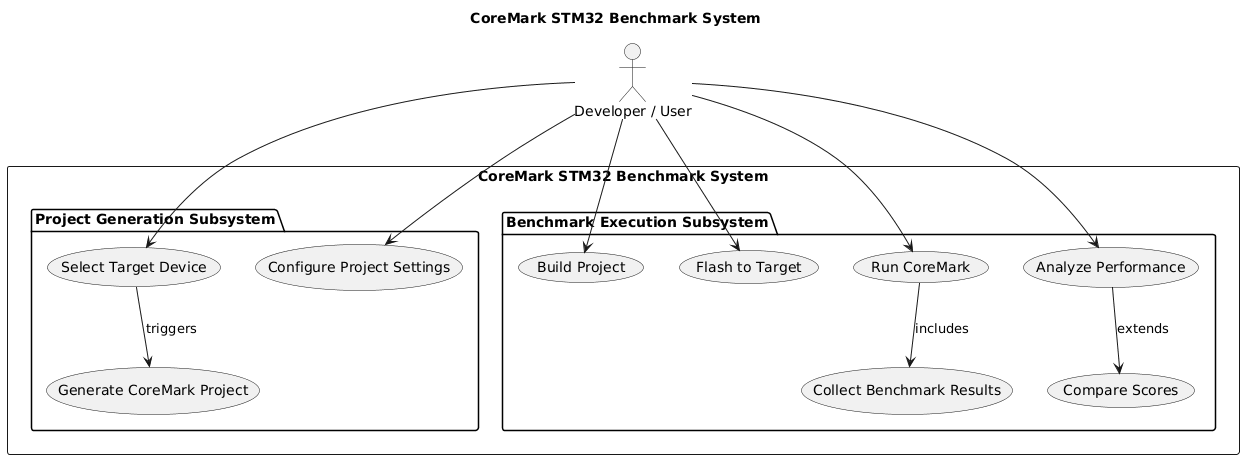
\includegraphics[width=15cm]{img/ST_Summer_Internship/use_case2.png}
	\caption{Automated CoreMark Benchmarking Use-Case Diagram}
	\label{fig:use_case_diagram}
\end{figure}

The Use-Case diagram in Figure \ref{fig:use_case_diagram} illustrates the interactions between a user, the project generation tool and the project's execution space.
Refer to Table \ref{tab:use_cases} for an in-depth explanation:

\begin{xltabular}{\linewidth}{@{}>{\bfseries}l X@{}}
	\caption{Automated CoreMark Benchmarking\label{tab:use_cases}} \\
	\toprule
	\textbf{Use Case} & \textbf{Relevance} \\
	\midrule
	\endfirsthead % Header for first page
	
	\multicolumn{2}{c}{{\tablename\ \thetable{} -- Continued from previous page}} \\
	\toprule
	\textbf{Use Case} & \textbf{Relevance} \\
	\midrule
	\endhead % Header for subsequent pages
	
	\midrule
	\multicolumn{2}{r}{{Continued on next page}} \\
	\endfoot % Footer for all pages except last
	
	\bottomrule
	\endlastfoot % Footer for the last page
	
	\multicolumn{2}{ c }{\textbf{Project Generation Subsystem}} \\
	\midrule
	Select Target Device &
	The developer selects the STM32 device or family for which the CoreMark project should be generated. 
	This ensures that the automation tool generates the correct configuration files and CMSIS device support. \\
	\midrule
	Configure Project Settings &
	The developer configures CoreMark-specific parameters such as iteration counts, seed values, and compiler optimization flags 
	before building and running the benchmark. \\
	\midrule
	Generate CoreMark Project &
	The automation tool generates a complete project structure, including the \texttt{csolution} files and necessary source code, 
	ready to be built and deployed for the selected STM32 target. \\
	\midrule
	\multicolumn{2}{ c }{\textbf{CoreMark Project Subsystem}} \\
	\midrule
	Build Project &
	The CoreMark project is compiled using the CMSIS build system and toolchain to produce a firmware image for the target hardware. \\
	\midrule
	Flash Target &
	The compiled binary is flashed to the STM32 device to prepare it for execution.\\
	\midrule
	Run CoreMark &
	The benchmark executes on the STM32 target, performing operations such as list processing, matrix manipulation, and state machine handling 
	to measure CPU performance. \\
	\midrule
	Collect CoreMark Results &
	During execution, CoreMark outputs the cycle count, execution time, and final score. \\
	\midrule
	Analyze Performance &
	The developer interprets the CoreMark/MHz score and other performance metrics to determine how well the device performs within the specified context. \\
	\midrule
	Compare Scores &
	Performance results are compared across different devices, toolchains, or configurations to guide hardware selection or optimization decisions.
\end{xltabular}

\section{Work Environment}
In this section, we outline the hardware and software resources utilized during the internship project that were essential for the development testing, and validation.

\subsection{Hardware Resources}
\begin{figure}[H]
	\centering
	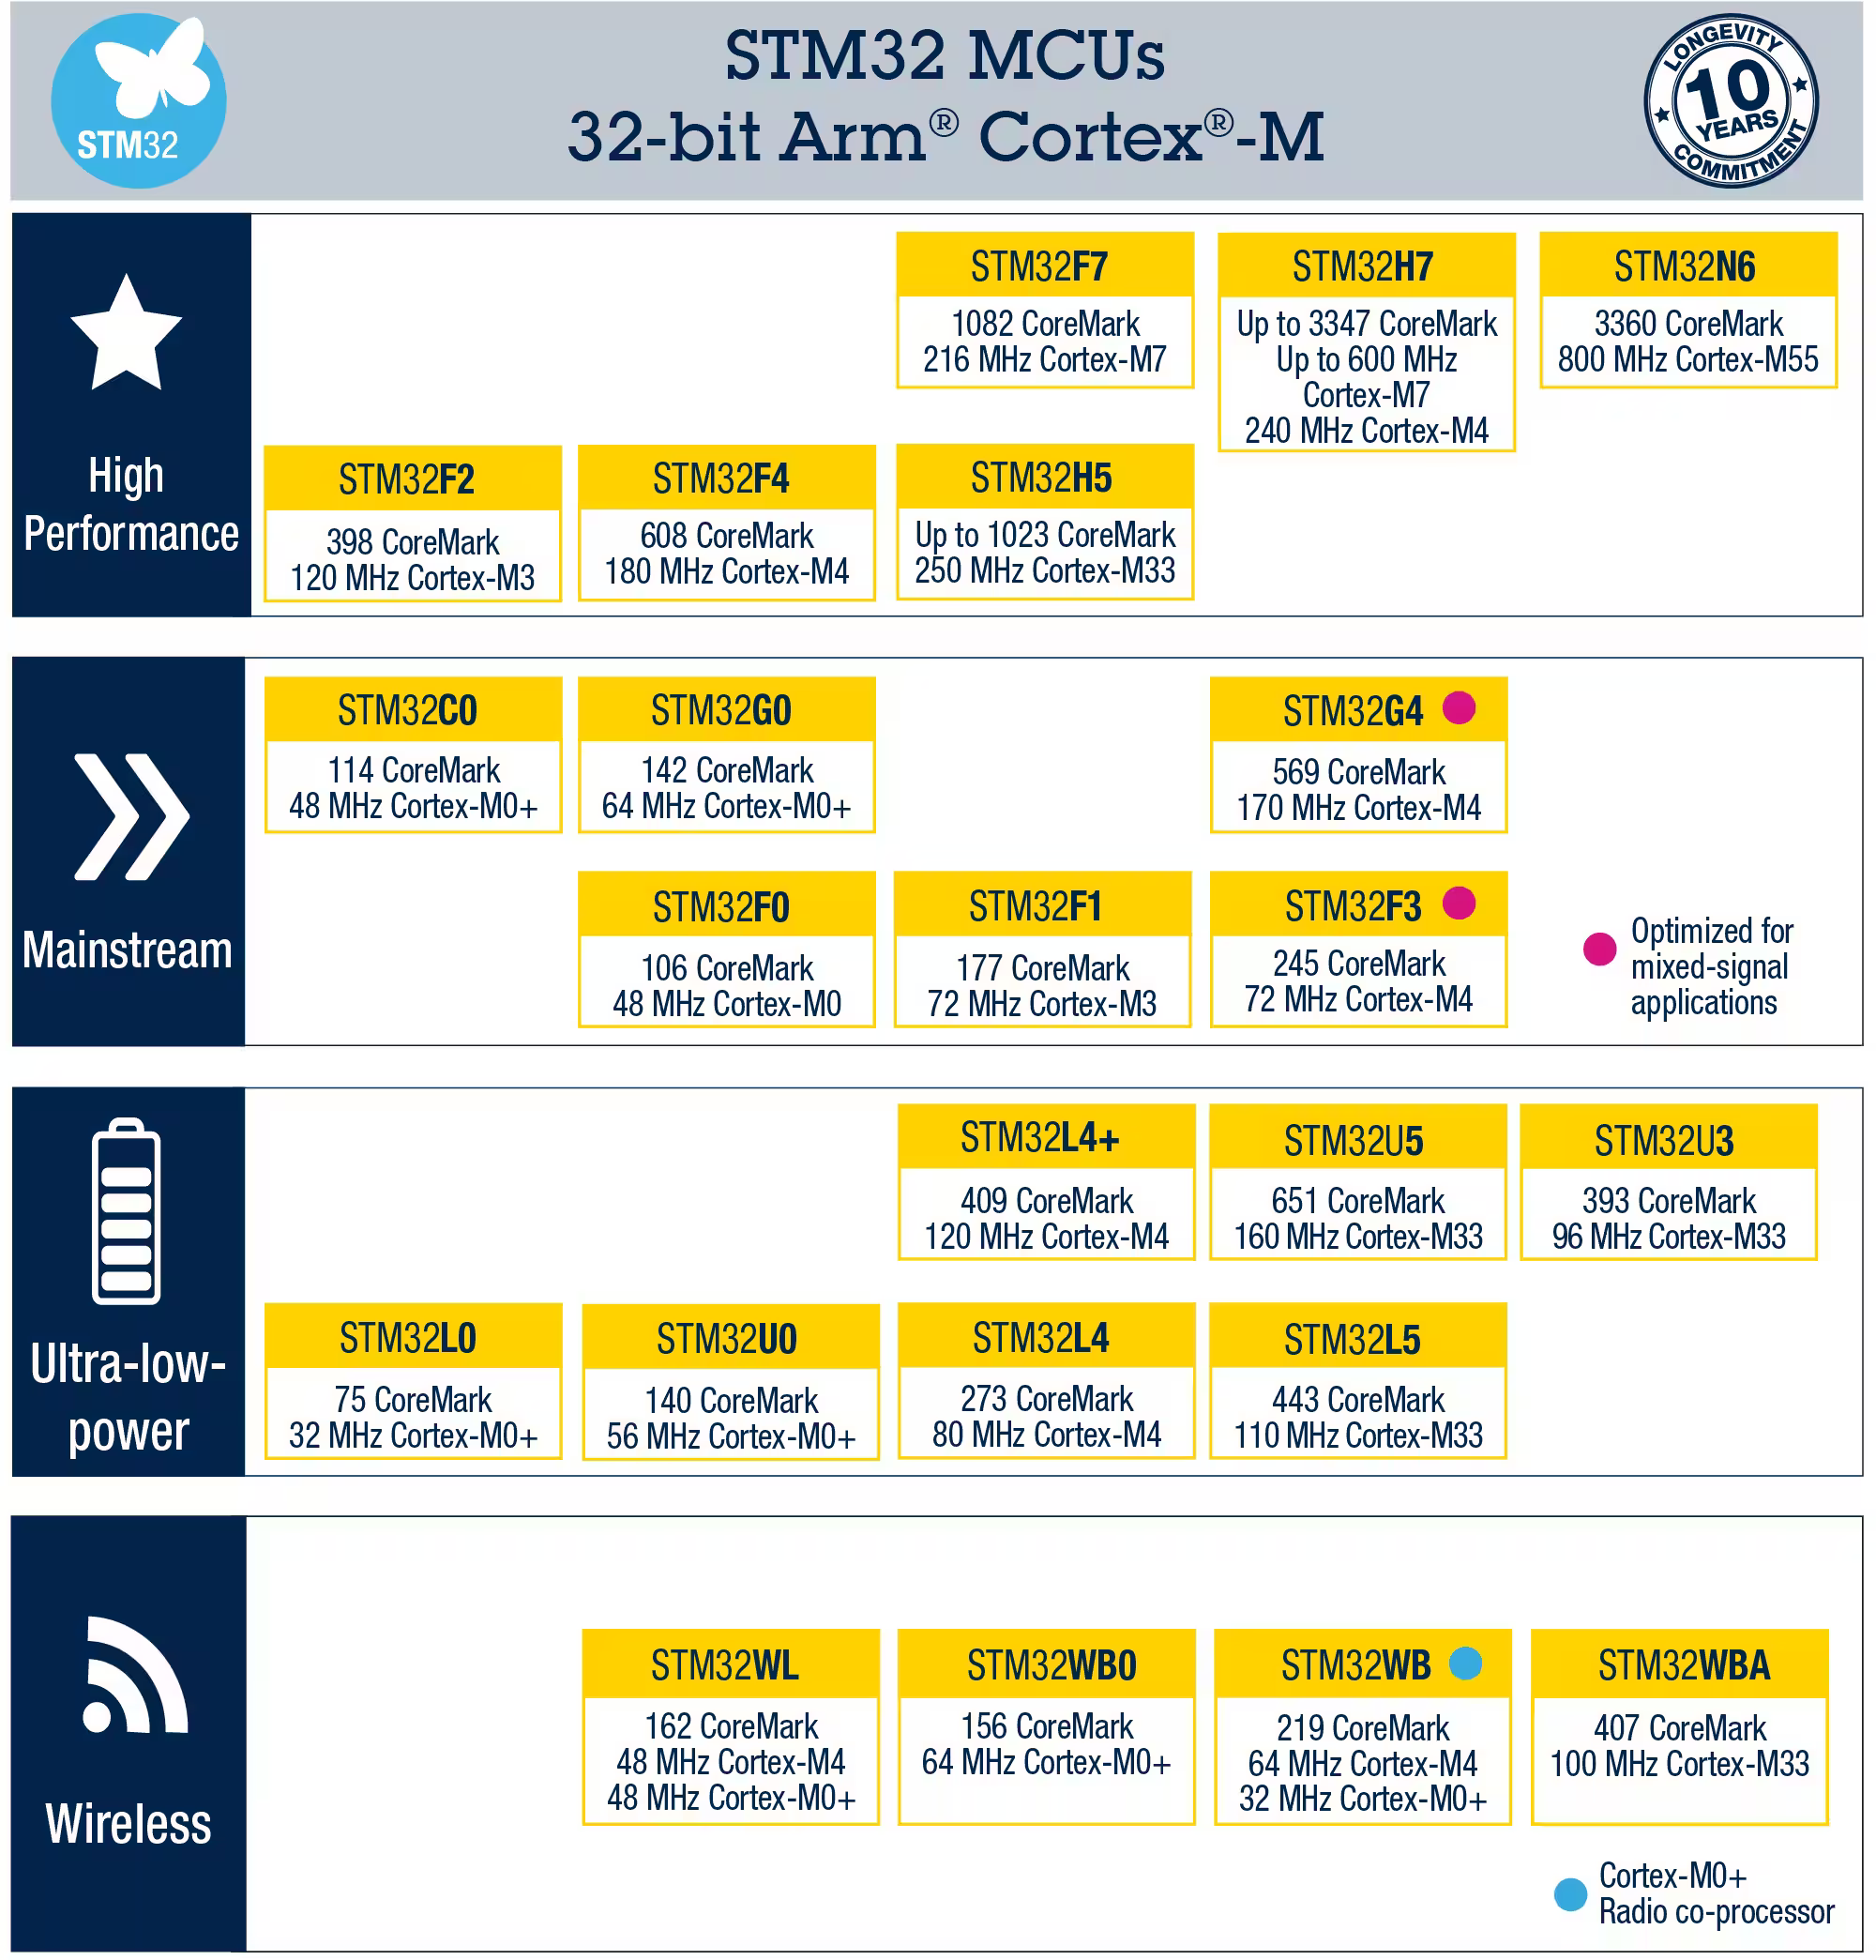
\includegraphics[width=15cm]{img/ST_Summer_Internship/arm_cortex_mcu_portfolio.png}
	\caption{STM32 Microcontroller Portfolio}
	\label{fig:stm32_portfolio}
\end{figure}
The project is meant to work on all STM32 MCUs, therefore as a base unit, the validation was done on a single board from all STM32 MCU families.
Table \ref{tab:stm32_mcu_families} describes all the available families:
\begin{xltabular}{\linewidth}{@{}>{\bfseries}l X@{} X@{} X@{} X@{} X@{}}
	\caption{STM32 Microcontroller Families\label{tab:stm32_mcu_families}} \\
	\toprule
	\textbf{Family} & \textbf{Core} & \textbf{Maximum Frequency(MHz)} & \textbf{Read-Only Memory} & \textbf{Random Access Memory} & \textbf{Additional Features} \\
	\midrule
	\endfirsthead % Header for first page
	
	\multicolumn{6}{c}{{\tablename\ \thetable{} -- Continued from previous page}} \\
	\toprule
	\textbf{Family} & \textbf{Core} & \textbf{Maximum Frequency} & \textbf{Read-Only Memory} & \textbf{Random Access Memory} & \textbf{Additional Features} \\
	\midrule
	\endhead % Header for subsequent pages
	
	\multicolumn{6}{r}{{Continued on next page}} \\
	\endfoot % Footer for all pages except last
	
	\bottomrule
	\endlastfoot % Footer for the last page
	
	STM32C0 &
	Arm Cortex-M0+ &
	48MHZ & 16-256KB & 6-36KB & - \\
	\midrule
	STM32F0 &
	Arm Cortex-M0 &
	48MHz & 16-256KB & 4-32KB & - \\
	\midrule
	STM32F1 &
	Arm Cortex-M3 &
	72MHz & 16KB-1MB & 4-96KB & - \\
	\midrule
	STM32F2 &
	Arm Cortex-M3 &
	120MHz & 128KB-1MB & 64KB-128KB & ART Accelerator \\
	\midrule
	STM32F3 &
	Arm Cortex-M4 &
	72MHz & 32-512KB & 16-80KB & CCM-SRAM and FPU/DFP instructions \\
	\midrule
	STM32F4 &
	Arm Cortex-M4 &
	180MHz & 64KB-2MB & 32-384KB & Chrom-ART Accelerator\\
	\midrule
	STM32F7 &
	Arm Cortex-M7 &
	216MHz & 64K-2MB & 256-512KB & L1 Data and Instruction Caches, TCM, Read-While-write Flash capabilities \\
	\midrule
	STM32G0 &
	Arm Cortex-M0+ &
	64MHz & 16-512KB & 8-144KB & \\
	\midrule
	STM32G4 &
	Arm Cortex-M4 &
	170MHz & 32-512KB & 32-128KB & CCM-SRAM and FPU/DFP instructions \\
	\midrule
	STM32H5 &
	Arm Cortex-M33 &
	250MHz & 128KB-2MB & 32-640KB & Integrated Instruction and Data Cache peripherals \\
	\midrule
	STM32H7 &
	Arm Cortex-M7 &
	600MHz & 64KB-2MB & 536KB-1.4MB & L1 Data and Instruction Cache, TCM, Chrome-ART and NeoChrom Accelerators.  \\
	\midrule
	STM32L0 &
	Arm Cortex-M0+ &
	32MHz & 8-192KB & 2-20KB & Up to 6KB of EEPROM \\
	\midrule
	STM32L1 &
	Arm Cortex-M3 &
	32MHz & 32-512KB & 4-80KB & Up to 16KB of EEPROM \\
	\midrule
	STM32L4 &
	Arm Cortex-M4 &
	80MHz & 64KB-1MB & 40-320KB & Chrom-ART Accelerator \\
	\midrule
	STM32L4+ &
	Arm Cortex-M4 &
	120MHz & 512KB-2MB & 320-640KB & Chrom-ART Accelerator \\
	\midrule
	STM32L5 &
	Arm Cortex-M33 &
	110MHz & 256-512MB & 256KB & ART Accelerator \\
	\midrule
	STM32N6 &
	Arm Cortex-M55 &
	800MHz & 0 & 4.2MB & Neural-ART Accelerator(Up to 1GHz Clock Speed) \\
	\midrule
	STM32U0 &
	Arm Cortex-M0+ &
	56MHz & 16-256KB & 12-40KB & - \\
	\midrule
	STM32U3 &
	Arm Cortex-M33 &
	96MHz & 512KB-1MB & 256KB & Integrated Instruction and Data Cache peripherals \\
	\midrule
	STM32U5 &
	Arm Cortex-M33 &
	160MHz & 128-4MB & 274KB-3MB & Integrated Instruction and Data Cache peripherals \\
	\midrule
	STM32WB &
	Arm Cortex-M4 &
	64MHz & 256KB-1MB & 48-256KB & - \\
	\midrule
	STM32WB0 &
	Arm Cortex-M0+ &
	64MHz & 192-512KB & 24-64KB & - \\
	\midrule
	STM32WBA &
	Arm Cortex-M33 &
	100MHz & 512KB-2MB & 64-512KB & Integrated Instruction and Data Cache peripherals \\
	\midrule
	STM32WL &
	Arm Cortex-M4 &
	64MHz & 64-256KB & 8-64KB & - \\
	
\end{xltabular}

\subsection{Software Resources}
The following software tools were used for the  development, debugging and testing of the project:
\subsection*{Programming Languages}
\begin{itemize}
	\item \textbf{C:}
	 C is a general-purpose programming language. By design, C gives the programmer relatively direct access to the features of the typical CPU architecture, customized for the target instruction set. It has been and continues to be used to implement operating systems (especially kernels), device drivers, and protocol stacks, and embedded applications. C is used on computers that range from the largest supercomputers to the smallest microcontrollers. 
	\item \textbf{Go:}
	 Go (or Golang) is a high-level general purpose programming language that is statically typed and compiled. It is known for the simplicity of its syntax and the efficiency of development that it enables by the inclusion of a large standard library supplying many needs for common projects.
	\item \textbf{Python:}
	 Python is a high-level, general-purpose programming language. Its design philosophy emphasizes code readability with the use of significant indentation.
	 Python is dynamically type-checked and garbage-collected. It supports multiple programming paradigms, including structured (particularly procedural), object-oriented and functional programming. 
\end{itemize}
\subsection*{Integrated Development Environments and Text Editors}
\subsubsection{Keil \textmu vision}
\subsubsection{IAR Embedded Workbench}
IAR Embedded Workbench is an integrated development environment (IDE) used for programming, debugging, and optimizing embedded applications. It provides comprehensive support for STM32 microcontrollers. Key features include:
\begin{itemize}
    \item Advanced debugging capabilities with breakpoints, watch windows, and real-time data visualization.
    \item Code optimization tools to improve performance and reduce memory footprint.
    \item Integrated support for STM32CubeMX, allowing seamless project setup and configuration.
\end{itemize}
\begin{figure}[H]
  \centering
  
\includegraphics[width=8cm]{img/IAR.png}
  \caption{IAR Embedded Workbench}
  \label{fig:IAR}
\end{figure}
\subsubsection{Visual Studio Code}
\subsection*{Embedded Systems Compiler Toolchains}
\subsubsection{GCC}
\subsubsection{ARM Compiler v6}
\subsubsection{IAR Toolchain}
\subsection*{Development Tools}
\subsubsection{CMake}
\subsubsection{CMSIS-Toolbox}
\begin{itemize}
	\item \textbf{csolution}
	\item \textbf{cproject}
	\item \textbf{cpackget}
\end{itemize}
\subsubsection{PyOCD}
\subsubsection{OpenOCD}
\subsubsection{STM32CubeProgrammer}
\subsubsection{STM32CubeMX}
STM32CubeMX is a graphical software configuration tool that simplifies the development of STM32-based applications. It allows developers to:
\begin{itemize}
	\item Configure microcontroller peripherals and middleware components through an intuitive graphical interface.
	\item Generate initialization code for STM32 microcontrollers, reducing development time.
	\item Integrate with various IDEs, including IAR Embedded Workbench, for a streamlined development workflow.
\end{itemize}
\begin{figure}[H]
	\centering
	
\includegraphics[width=8cm]{img/CUBEMX.jpg}
	\caption{STM32CubeMX}
	\label{fig:mx}
\end{figure}
\section*{Conclusion}
The work environment for this internship includes both hardware and software resources that are essential for the successful implementation of the project.
